\chapter{Quadratic Programming}
\label{chap:quadratic-programming}

\section{Introduction}

A general quadratic program (QP) is written in the form:
\begin{equation}
    \min_{x \in \mathbb{R}^n} q(x) = \frac{1}{2} x^\top G x + c^\top x,
\end{equation}
subject to the constraints:
\begin{align}
    a_i^\top x &= b_i, \quad i \in \mathcal{E}, \\
    a_i^\top x &\geq b_i, \quad i \in \mathcal{I},
\end{align}
where $G$ is an $n \times n$ symmetric matrix, $c \in \mathbb{R}^n$, $a_i \in \mathbb{R}^n$ and $b_i \in \mathbb{R}$.

\begin{remarque}
    For QPs, a finite amount of computation is required to solve them or to declare them infeasible.
    \begin{itemize}
        \item We speak of a \textbf{convex QP} when $G$ is positive semi-definite.
        \item We speak of a \textbf{strictly convex QP} when $G$ is positive definite.
    \end{itemize}
\end{remarque}

\section{QP with Equality Constraints}

Consider problems of the form:
\begin{equation}
    \min_{x \in \mathbb{R}^n} \frac{1}{2} x^\top G x + c^\top x, \quad \text{subject to} \quad Ax = b,
\end{equation}
where $A \in \mathbb{R}^{m \times n}$ (with $m < n$) is the Jacobian of the constraints. Its rows are the vectors $a_i$. The vector $b \in \mathbb{R}^m$ gathers the scalars $b_i$.
We assume that the matrix $A$ has \textbf{full rank}.

\subsection{Properties}

The first-order optimality conditions (KKT) are written as:
\begin{equation}
    \begin{cases}
        G x^* + c - A^\top \lambda^* = 0 \\
        A x^* = b
    \end{cases}
\end{equation}
This is equivalent to the following matrix system:
\begin{equation}
    \begin{pmatrix}
        G & -A^\top \\
        A & 0
    \end{pmatrix}
    \begin{pmatrix}
        x^* \\
        \lambda^*
    \end{pmatrix}
    =
    \begin{pmatrix}
        -c \\
        b
    \end{pmatrix}
\end{equation}

\begin{remarque}
    If we rewrite $x^*$ as $x + p$, where $x$ is a candidate for the solution and $p$ is a step, the system becomes:
    \begin{equation}
        \begin{pmatrix}
            G & A^\top \\
            A & 0
        \end{pmatrix}
        \begin{pmatrix}
            -p \\
            \lambda^*
        \end{pmatrix}
        =
        \begin{pmatrix}
            g \\
            h
        \end{pmatrix}
    \end{equation}
    where $g = c + Gx$ is the gradient of the objective function at point $x$, $h = Ax - b$ is the residual of the constraints, and $p = x^* - x$.
    
    The matrix $\begin{pmatrix} G & A^\top \\ A & 0 \end{pmatrix}$ is called the \textbf{KKT matrix}.
\end{remarque}

Let $Z$ be an $n \times (n-m)$ matrix whose columns form a basis for the null-space of $A$. That is, $AZ = 0$ and $A$ has full rank.

\begin{lemme}
    Assume that $A$ has full row rank. Assume that the reduced Hessian matrix $Z^\top G Z$ is positive definite.
    Then the KKT matrix $\begin{pmatrix} G & A^\top \\ A & 0 \end{pmatrix}$ is non-singular.
\end{lemme}

\begin{proof}
    Let the vectors $w$ and $v$ be such that:
    \begin{equation}
        \begin{pmatrix}
            G & A^\top \\
            A & 0
        \end{pmatrix}
        \begin{pmatrix}
            w \\
            v
        \end{pmatrix}
        = 0
    \end{equation}
    The second block of rows gives $Aw = 0$. Thus, $w$ belongs to the null space of $A$, so there exists a vector $u$ such that $w = Zu$.
    
    Multiply the first block of rows by $w^\top$ from the left:
    \begin{align*}
        0 &= \begin{pmatrix} w \\ v \end{pmatrix}^\top \begin{pmatrix} G & A^\top \\ A & 0 \end{pmatrix} \begin{pmatrix} w \\ v \end{pmatrix} \\
          &= w^\top G w + w^\top A^\top v + v^\top A w
    \end{align*}
    Since $Aw = 0$, we have $v^\top A w = 0$. Similarly, $w^\top A^\top v = (Aw)^\top v = 0$.
    Thus we obtain $0 = w^\top G w$.
    Replacing $w$ by $Zu$, we get:
    \begin{equation}
        0 = (Zu)^\top G (Zu) = u^\top (Z^\top G Z) u
    \end{equation}
    Since $Z^\top G Z$ is positive definite, this implies that $u = 0$, and consequently $w = Zu = 0$.
    
    The first block of rows then becomes $G \cdot 0 + A^\top v = 0$, i.e., $A^\top v = 0$.
    Since $A$ has full row rank, $A^\top$ has full column rank, which implies that $v = 0$.
    
    Therefore, the only solution vector is the zero vector $\begin{pmatrix} w \\ v \end{pmatrix} = 0$, which proves that the matrix is non-singular.
\end{proof}

We will prove that under the same conditions, $x^*$ is a strict local minimizer, and even a global solution.

\begin{theoreme}
    Assume that $A$ has full row rank. Assume that the reduced Hessian matrix $Z^\top G Z$ is positive definite.
    Then the vector $x^*$ satisfying
    \begin{equation}
        \begin{pmatrix}
            G & -A^\top \\
            A & 0
        \end{pmatrix}
        \begin{pmatrix}
            x^* \\
            \lambda^*
        \end{pmatrix}
        =
        \begin{pmatrix}
            -c \\
            b
        \end{pmatrix}
    \end{equation}
    is the unique global solution.
\end{theoreme}

\begin{proof}
    Let $x$ be another feasible point: $Ax = b$.
    Let $p = x^* - x$.
    Since $Ax = b$ and $Ax^* = b$, we have
    \begin{equation}
        Ap = A(x^* - x) = 0.
    \end{equation}
    Substitute into $q(x)$:
    \begin{align*}
        q(x) = q(x^* - p) &= \frac{1}{2} (x^* - p)^\top G (x^* - p) + c^\top (x^* - p) \\
                          &= \frac{1}{2} p^\top G p - p^\top G x^* + \frac{1}{2} (x^*)^\top G x^* - c^\top p + c^\top x^* \\
                          &= \frac{1}{2} p^\top G p - p^\top G x^* - c^\top p + q(x^*) \quad (*)
    \end{align*}
    Now use the first block of rows of the KKT system:
    \begin{equation}
        G x^* + c - A^\top \lambda^* = 0 \implies G x^* + c = A^\top \lambda^*
    \end{equation}
    Multiply from the left by $p^\top$:
    \begin{equation}
        p^\top (G x^* + c) = p^\top A^\top \lambda^* = (Ap)^\top \lambda^*
    \end{equation}
    But we have seen that $Ap = 0$, so the right-hand side is zero. Thus:
    \begin{equation}
        p^\top G x^* + p^\top c = 0 \implies -p^\top G x^* - c^\top p = 0
    \end{equation}
    Substituting this into equation (*), we obtain:
    \begin{equation}
        q(x) = q(x^*) + \frac{1}{2} p^\top G p
    \end{equation}
    Since $p$ is in the null space of $A$, there exists a vector $u \in \mathbb{R}^{n-m}$ such that $p = Zu$. Then:
    \begin{equation}
        p^\top G p = (Zu)^\top G (Zu) = u^\top (Z^\top G Z) u
    \end{equation}
    Since the reduced Hessian matrix $Z^\top G Z$ is assumed positive definite, we have $u^\top Z^\top G Z u > 0$ for all $u \neq 0$.
    But $u \neq 0 \iff p \neq 0 \iff x \neq x^*$.
    
    Consequently, for every feasible $x \neq x^*$,
    \begin{equation}
        q(x) = q(x^*) + \frac{1}{2} u^\top Z^\top G Z u > q(x^*)
    \end{equation}
    Which proves that $x^*$ is the unique global minimizer.
\end{proof}

\subsection{Direct Solution of the KKT System}

\begin{remarque}
    It can be proven (Forsgren et al.) that the KKT matrix is always indefinite when $m \ge 1$. In other words, there exist vectors $x$ and $y$ such that $x^\top K x > 0$ and $y^\top K y < 0$ (where $K$ denotes the KKT matrix).
\end{remarque}

\subsubsection{Factorization of the Full KKT System}

We cannot use Cholesky factorization due to the indefinite nature of the matrix.
An LU decomposition is feasible, but it ignores the symmetry of the system.

Thus, we use the \textbf{symmetric indefinite factorization} for $K$ (symmetric matrix):
\begin{equation}
    P K P^\top = L B L^\top,
\end{equation}
where:
\begin{itemize}
    \item $P$ is a permutation matrix;
    \item $L$ is a unit lower triangular matrix;
    \item $B$ is a block-diagonal matrix, with blocks of size $1 \times 1$ or $2 \times 2$.
\end{itemize}

To solve the KKT system $K \begin{pmatrix} -p \\ \lambda^* \end{pmatrix} = \begin{pmatrix} g \\ h \end{pmatrix}$:
\begin{enumerate}
    \item Solve $Lz = P^\top \begin{pmatrix} g \\ h \end{pmatrix}$ for $z$ (forward substitution).
    \item Solve $B\hat{z} = z$ for $\hat{z}$ (block-diagonal solve).
    \item Solve $L^\top \bar{z} = \hat{z}$ for $\bar{z}$ (backward substitution).
    \item Set $\begin{pmatrix} -p \\ \lambda^* \end{pmatrix} = P \bar{z}$.
\end{enumerate}

\subsubsection{Schur Complement Method}

This method is applicable if $G$ is \textbf{positive definite} (and thus invertible).
Starting from the KKT system:
\begin{equation}
    \begin{cases}
        -Gp + A^\top \lambda^* = g \\
        Ap = h
    \end{cases}
\end{equation}
Multiply the first equation by $AG^{-1}$:
\begin{align*}
    -AG^{-1}Gp + AG^{-1}A^\top \lambda^* &= AG^{-1}g \\
    -Ap + (AG^{-1}A^\top) \lambda^* &= AG^{-1}g
\end{align*}
Using the second equation ($Ap=h$), we obtain:
\begin{equation}
    (AG^{-1}A^\top) \lambda^* = AG^{-1}g - h
\end{equation}
The system $(AG^{-1}A^\top) \lambda^* = AG^{-1}g - h$ is positive definite. We can solve it to find $\lambda^*$.
Next, we use the first block of rows of the KKT system to find $p$:
\begin{equation}
    Gp = A^\top \lambda^* - g \implies p = G^{-1}(A^\top \lambda^* - g).
\end{equation}

\paragraph{Numerical considerations:}
This method requires operations with $G^{-1}$ and the factorization of the matrix $AG^{-1}A^\top$. It is therefore suitable when:
\begin{itemize}
    \item $G$ is well-conditioned and easy to invert (example: diagonal).
    \item $G^{-1}$ is explicitly known.
    \item $m$ (the number of constraints) is small.
\end{itemize}

\subsubsection{Null-Space Method}

The non-singularity of $G$ is not required here; we only need the assumptions of the lemma ($A$ full rank, $Z^\top G Z$ positive definite).
Suppose we partition the vector $p$ as follows:
\begin{equation}
    p = Y p_Y + Z p_Z
\end{equation}
where $Z$ is the $n \times (n-m)$ matrix of the null space of $A$, and $Y$ is an $n \times m$ matrix such that the matrix $[Y \mid Z]$ is non-singular.
For simplification, we often choose $Y$ such that $AY = I$ (if possible) or $A [Y \mid Z]$ is triangular.

Substitute $p$ into the second equation of the KKT system ($Ap = h$):
\begin{equation}
    A(Y p_Y + Z p_Z) = h \implies AY p_Y + AZ p_Z = h
\end{equation}
Since $Z$ is in the null space, $AZ = 0$. Thus:
\begin{equation}
    (AY) p_Y = h
\end{equation}
Since $A$ has rank $m$ and $[Y \mid Z]$ is non-singular, the matrix $AY$ is non-singular of size $m \times m$.
We can therefore solve this system to find $p_Y$. (If we choose $Y$ such that $AY=I$, then $p_Y = h$).

Next, substitute $p$ into the first equation of the KKT system ($ -Gp + A^\top \lambda^* = g $):
\begin{equation}
    -G(Y p_Y + Z p_Z) + A^\top \lambda^* = g
\end{equation}
Multiply from the left by $Z^\top$:
\begin{align*}
    -Z^\top G Y p_Y - Z^\top G Z p_Z + Z^\top A^\top \lambda^* &= Z^\top g \\
    -Z^\top G Y p_Y - Z^\top G Z p_Z + (AZ)^\top \lambda^* &= Z^\top g
\end{align*}
Since $AZ=0$, the term involving $\lambda^*$ disappears:
\begin{equation}
    -(Z^\top G Z) p_Z = Z^\top g + Z^\top G Y p_Y
\end{equation}
The system $(Z^\top G Z) p_Z = -(Z^\top g + Z^\top G Y p_Y)$ allows us to find $p_Z$, because the reduced matrix $Z^\top G Z$ is assumed positive definite (hence invertible).

Finally, to find $\lambda^*$, we multiply the first equation by $Y^\top$:
\begin{equation}
    (AY)^\top \lambda^* = Y^\top (g + Gp)
\end{equation}
This linear system allows us to determine $\lambda^*$.

\paragraph{Remarks:}
\begin{itemize}
    \item This method is efficient when $n-m$ is small.
    \item Computing $Z$ is the main difficulty; it is not unique. Poor choices can result in poor conditioning of $Z^\top G Z$.
\end{itemize}

\paragraph{Example:}
Let $G = \begin{pmatrix} 6 & 2 & 1 \\ 2 & 5 & 2 \\ 1 & 2 & 4 \end{pmatrix}$, $c = \begin{pmatrix} -8 \\ -3 \\ -3 \end{pmatrix}$. Constraints: $\begin{cases} x_1 + x_3 = 3 \\ x_2 + x_3 = 0 \end{cases}$.
Hence $A = \begin{pmatrix} 1 & 0 & 1 \\ 0 & 1 & 1 \end{pmatrix}$ and $b = \begin{pmatrix} 3 \\ 0 \end{pmatrix}$.
We can choose $Z = \begin{pmatrix} -1 \\ -1 \\ 1 \end{pmatrix}$ (verify $AZ=0$) and $Y = \begin{pmatrix} 2/3 & -1/3 \\ -1/3 & 2/3 \\ 1/3 & 1/3 \end{pmatrix}$ such that $AY = I_2$.

\paragraph{Example (continued):}
Let $x = \begin{pmatrix} -1 \\ -2 \\ 2 \end{pmatrix}$.
We compute $h = Ax - b = \begin{pmatrix} 0 \\ 0 \end{pmatrix}$ and $g = c + Gx = \begin{pmatrix} -7/2 \\ -2 \\ 2 \end{pmatrix}$ (note: values from the course example).

\begin{enumerate}
    \item \textbf{Find $p_Y$}: Solve $(AY) p_Y = -h$. Here $p_Y = -h = \begin{pmatrix} 0 \\ 0 \end{pmatrix}$.
    \item \textbf{Find $p_Z$}: Solve $(Z^\top G Z) p_Z = -(Z^\top g + Z^\top G Y p_Y)$.
    Let's compute the terms: 
    $Z^\top G Z = \begin{pmatrix} -1 & -1 & 1 \end{pmatrix} \begin{pmatrix} 6 & 2 & 1 \\ 2 & 5 & 2 \\ 1 & 2 & 4 \end{pmatrix} \begin{pmatrix} -1 \\ -1 \\ 1 \end{pmatrix} = 13$ (scalar).
    $Z^\top g = -13$.
    The term $Z^\top G Y p_Y$ is zero since $p_Y = 0$.
    The equation becomes: $13 p_Z = -(-13) \implies p_Z = 1$.
    \item \textbf{Reconstruct $p$}:
    $p = Y p_Y + Z p_Z = Y \cdot 0 + Z \cdot 1 = \begin{pmatrix} -1 \\ -1 \\ 1 \end{pmatrix}$.
    \item \textbf{Solution}:
    $x^* = x + p = \begin{pmatrix} -1 \\ -2 \\ 2 \end{pmatrix} + \begin{pmatrix} -1 \\ -1 \\ 1 \end{pmatrix} = \begin{pmatrix} -2 \\ -3 \\ 3 \end{pmatrix}$.
\end{enumerate}

\subsection{Iterative Solution of the KKT System}

For large systems, direct methods become too expensive. Iterative methods, such as Conjugate Gradient (CG), are then preferred.
However, using CG directly on the full KKT system is unstable because the KKT matrix is not positive definite (it is indefinite).

The idea is to apply CG on the \textbf{reduced system}, which is positive definite (under the assumption that $Z^\top G Z$ is).

Substitute $x^* = Y p_Y + Z p_Z$ into the problem.
$p_Z$ is the solution to the unconstrained minimization problem:
\begin{equation}
    \min_{p_Z \in \mathbb{R}^{n-m}} \frac{1}{2} p_Z^\top (Z^\top G Z) p_Z + p_Z^\top c_Z
\end{equation}
where $c_Z = Z^\top G Y p_Y + Z^\top c$ (noting that the linear term also depends on $p_Y$, which is determined by the constraints).

Thus, $p_Z$ satisfies the normal equation:
\begin{equation}
    (Z^\top G Z) p_Z = -c_Z
\end{equation}
Since $Z^\top G Z$ is positive definite, we can use the Conjugate Gradient (CG) to find $p_Z$.

\paragraph{Preconditioning:}
In practice, a preconditioner $W_{ZZ}$ is used to accelerate convergence. A good preconditioner should cluster the eigenvalues of $W_{ZZ}^{-1/2} (Z^\top G Z) W_{ZZ}^{-1/2}$.
Ideally, one would choose $W_{ZZ} = Z^\top G Z$, but this is too expensive.
Good choices are of the form $W_{ZZ} = Z^\top H Z$, where $H$ is a symmetric approximation of $G$ such that $Z^\top H Z$ is positive definite.

The following algorithm (Algorithm 17 in some references) describes this procedure:

\begin{algorithm}[H]
    \caption{Preconditioned Conjugate Gradient for reduced systems}
    \SetAlgoLined
    Choose an initial point $x_Z$ (corresponding to our $p_Z$)\;
    Compute $r_Z=Z^\top GZx_Z + c_Z$, $g_Z=W_{ZZ}^{-1}r_Z$, and $d_Z=-g_Z$\;
    \Repeat{a termination test is satisfied}{
        $\alpha\leftarrow \frac{r_Z^\top g_Z}{d_Z^\top Z^\top GZd_Z}$\;
        $x_Z\leftarrow x_Z+\alpha d_Z$\;
        $r_Z^+\leftarrow r_Z + \alpha Z^\top GZd_Z$\;
        $g_Z^+\leftarrow W_{ZZ}^{-1}r_Z^+$\;
        $\beta \leftarrow \frac{(r_Z^+)^\top g_Z^+}{r_Z^\top g_Z}$\;
        $d_Z\leftarrow -g_Z^++\beta d_Z$\;
        $g_Z\leftarrow g_Z^+$\;
        $r_Z\leftarrow r_Z^+$\;
    }
\end{algorithm}

\section{Problems with Inequality Constraints}

\subsection{Properties}


Consider the following optimization problem:
    \begin{equation}
        \min_{x \in \mathbb{R}^n} \frac{1}{2} x^\top G x + c^\top x \quad \text{subject to} \quad
        \begin{cases}
            a_i^\top x - b_i \ge 0, & \forall i \in \mathcal{I} \\
            a_i^\top x - b_i = 0, & \forall i \in \mathcal{E}
        \end{cases}
    \end{equation}

    The Lagrangian is defined by:
    \begin{equation}
        \mathcal{L}(x, \lambda) = \frac{1}{2} x^\top G x + c^\top x - \sum_{i \in \mathcal{E} \cup \mathcal{I}} \lambda_i (a_i^\top x - b_i)
    \end{equation}

    Recall the active set:
    \begin{equation}
        \mathcal{A}(x) = \{ i \in \mathcal{E} \cup \mathcal{I} \mid a_i^\top x - b_i = 0 \}
    \end{equation}

    \paragraph{KKT Conditions:}
    Any solution $x^*$ satisfies, for some multipliers $\lambda_i^*$:
    \begin{equation}
        \begin{cases}
            G x^* + c - \sum_{i \in \mathcal{E} \cup \mathcal{I}} \lambda_i^* a_i = 0 \\
            a_i^\top x^* - b_i \ge 0, \quad \forall i \in \mathcal{I} \setminus \mathcal{A}(x^*) \\
            a_i^\top x^* - b_i = 0, \quad \forall i \in \mathcal{E} \\
            \lambda_i^* \ge 0, \quad \forall i \in \mathcal{I} \cap \mathcal{A}(x^*)
        \end{cases}
    \end{equation}
    \emph{Note:} In the system, feasibility conditions are implicitly noted by the index sets, and the complementarity condition is summarized by $\lambda_i^* \ge 0$ for active inequality constraints (and $\lambda_i^* = 0$ for inactive ones).

    \begin{remarque}
        We do not need to assume linear independence constraint qualification (LICQ) because the constraints are linear. We merely assume that the matrix $A$ of equality constraints has full row rank.
    \end{remarque}

    \begin{theoreme}
        If $x^*$ satisfies the KKT conditions for some $\lambda^*$, and if $G$ is positive semi-definite, then $x^*$ is a global solution to the problem.
    \end{theoreme}

    \begin{proof}
        Let $x$ be another feasible point. We have:
        \begin{equation}
            \begin{aligned}
                a_i^\top x &= b_i, \quad \forall i \in \mathcal{E} \\
                a_i^\top x &\ge b_i, \quad \forall i \in \mathcal{I}
            \end{aligned}
        \end{equation}
        Thus, considering the difference with $x^*$:
        \begin{equation}
            \begin{aligned}
                a_i^\top (x - x^*) &= 0, \quad \forall i \in \mathcal{E} \\
                a_i^\top (x - x^*) &\ge 0, \quad \forall i \in \mathcal{I} \cap \mathcal{A}(x^*)
            \end{aligned}
        \end{equation}
        The second inequality comes from the fact that for $i \in \mathcal{A}(x^*)$, $a_i^\top x^* = b_i$, so $a_i^\top x \ge b_i \implies a_i^\top (x - x^*) \ge 0$.

        From the first KKT condition:
        \begin{equation}
            (G x^* + c) = \sum_{i \in \mathcal{E} \cup \mathcal{I}} \lambda_i^* a_i
        \end{equation}
        Multiply by $(x - x^*)^\top$:
        \begin{equation}
            (x - x^*)^\top (G x^* + c) = \sum_{i \in \mathcal{E} \cup \mathcal{I}} \lambda_i^* a_i^\top (x - x^*)
        \end{equation}
        Let's decompose the sum:
        \begin{equation}
            \sum_{i \in \mathcal{E}} \lambda_i^* \underbrace{a_i^\top (x - x^*)}_{=0} + \sum_{i \in \mathcal{I} \cap \mathcal{A}(x^*)} \underbrace{\lambda_i^*}_{\ge 0} \underbrace{a_i^\top (x - x^*)}_{\ge 0} + \sum_{i \in \mathcal{I} \setminus \mathcal{A}(x^*)} \underbrace{\lambda_i^*}_{=0} a_i^\top (x - x^*)
        \end{equation}
        All terms are zero or positive. Therefore:
        \begin{equation}
            (x - x^*)^\top (G x^* + c) \ge 0
        \end{equation}

        Now consider the Taylor series expansion (exact for a quadratic) of $q(x)$ around $x^*$:
        \begin{equation}
            q(x) = q(x^*) + (x - x^*)^\top \nabla q(x^*) + \frac{1}{2} (x - x^*)^\top \nabla^2 q(x^*) (x - x^*)
        \end{equation}
        Now $\nabla q(x^*) = G x^* + c$ and $\nabla^2 q(x^*) = G$.
        \begin{equation}
            q(x) = q(x^*) + \underbrace{(x - x^*)^\top (G x^* + c)}_{\ge 0} + \frac{1}{2} \underbrace{(x - x^*)^\top G (x - x^*)}_{\ge 0 \text{ since } G \succeq 0}
        \end{equation}
        Thus, $q(x) \ge q(x^*)$, which proves that $x^*$ is a global solution.
    \end{proof}

    \begin{remarque}
        If $G$ is positive definite, the proof can be adapted to show that $x^*$ is unique.
        (Indeed, if $x \neq x^*$, the quadratic term is strictly positive).
    \end{remarque}


\begin{remarque}
    There are methods for general quadratic problems, for example:
    \begin{itemize}
        \item "Active-set" methods (Gould);
        \item Interior point methods (Wright or Vanderbei).
    \end{itemize}
\end{remarque}

\begin{figure}[H]
\centering
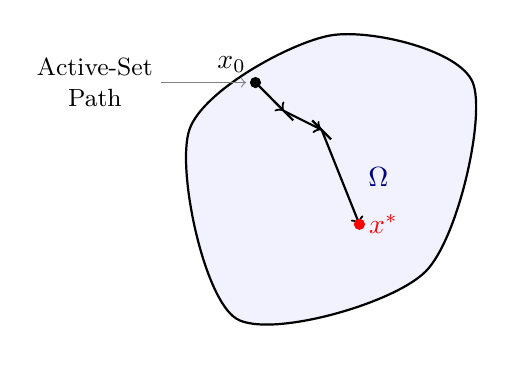
\begin{tikzpicture}[scale=1.2]
    \draw[thick, fill=blue!5] plot [smooth cycle] coordinates {(0,0) (2,0.5) (2.5,2.5) (1,3) (-0.5,2)};
    \node[blue!50!black] at (1.5, 1.5) {$\Omega$};
    
    \coordinate (x0) at (0.2, 2.5); 
    \filldraw[black] (x0) circle (1.5pt) node[above left] {$x_0$};
    
    \draw[thick, ->] (x0) -- (0.5, 2.2);
    \draw[thick] (0.4, 2.3) -- (0.6, 2.1); % Tick
    
    \draw[thick, ->] (0.5, 2.2) -- (0.9, 2.0);
    \draw[thick] (0.8, 2.1) -- (1.0, 1.9); % Tick
    
    \draw[thick, ->] (0.9, 2.0) -- (1.3, 1.0); % Moving towards interior or along boundary
    
    \filldraw[red] (1.3, 1.0) circle (1.5pt) node[right] {$x^*$};
    
    % Annotation "Active Set"
    \node[align=center, font=\small] at (-1.5, 2.5) {Active-Set\\Path};
    \draw[->, gray] (-0.8, 2.5) -- (0.1, 2.5);
    
\end{tikzpicture}
\caption{Illustration of an Active-Set type method for a general QP problem. The algorithm moves on the surface of the feasible set $\Omega$, activating or deactivating constraints until finding the optimum.}
\label{fig:generic-active-set}
\end{figure}

\begin{figureexplanation}
\textbf{General Active-Set Methods:}
Unlike the simple case of bounds, the region $\Omega$ can have a complex polyhedral shape defined by general linear inequalities.
The algorithm maintains a set of "active" (tight) constraints and moves on the corresponding boundary. If the gradient indicates that the objective function can be reduced by "taking off" from a constraint, it is relaxed (removed from the active set).
\end{figureexplanation}

We restrict our attention to problems with **bound constraints**:
\begin{equation}
    \min_{x \in \mathbb{R}^n} \frac{1}{2} x^\top G x + c^\top x \quad \text{subject to} \quad l \le x \le u
\end{equation}
where $G$ is symmetric, and $l, u \in \mathbb{R}^n$. The inequalities are understood component-wise ($l_i \le x_i \le u_i$). Some components of $l$ and $u$ can be $-\infty$ or $+\infty$.

The feasible region looks like a "box".

\begin{center}
\begin{tikzpicture}
    \draw[->] (-1,0) -- (4,0) node[right] {$x_1$};
    \draw[->] (0,-1) -- (0,4) node[above] {$x_2$};
    
    % Box
    \draw[blue, thick] (1,1) rectangle (3,3);
    
    \node at (1, -0.3) {$l_1$};
    \node at (3, -0.3) {$u_1$};
    \node at (-0.3, 1) {$l_2$};
    \node at (-0.3, 3) {$u_2$};
    \node at (2, 2) {$\mathcal{F}$};
\end{tikzpicture}
\captionof{figure}{Feasible Region (Box)}
\end{center}

\begin{figureexplanation}
\textbf{Geometry of bound constraints:}
The feasible set is a hyper-rectangle (box). For each dimension $i$, the variable $x_i$ is constrained to stay in the interval $[l_i, u_i]$.
The "projection" onto this set is very simple: if a coordinate exceeds a bound, it is simply brought back to the value of the bound (clipping).
\end{figureexplanation}

The iterations consist of two steps:

\subsubsection{Step 1: Computation of the Cauchy Point}

\paragraph{Projection onto the feasible region:}
The projection of a point $x$ onto the box $[l, u]$ is defined component by component:
\begin{equation}
    P(x, l, u)_i = \begin{cases}
        l_i & \text{if } x_i < l_i \\
        x_i & \text{if } l_i \le x_i \le u_i \\
        u_i & \text{if } x_i > u_i
    \end{cases}
\end{equation}

\paragraph{Piecewise linear path:}
The path $x(t)$, starting from the current iterate $x$, is defined by:
\begin{equation}
    x(t) = P(x - tg, l, u)
\end{equation}
where $g = Gx + c$ is the gradient.

This path follows the direction of steepest descent $-g$ and "bends" when it reaches a bound, thus remaining feasible. The first local minimum along this path is the \textbf{Cauchy Point} $x^c$.

\paragraph{Computation of the Cauchy Point:}
$x^c$ is the first local minimizer of $q(x(t))$. To find it, let's examine the \textbf{breakpoints}.

\textbf{1) Identify the $t$ at which the components of $x(t)$ reach a bound along $-g$:}

The value $\bar{t}_i$ for each component is:
\begin{equation}
    \bar{t}_i = \begin{cases}
        \displaystyle\frac{x_i - u_i}{g_i} & \text{if } g_i < 0 \text{ and } u_i < +\infty \\[10pt]
        \displaystyle\frac{x_i - l_i}{g_i} & \text{if } g_i > 0 \text{ and } l_i > -\infty \\[10pt]
        +\infty & \text{otherwise}
    \end{cases}
\end{equation}

The components of $x(t)$ then evolve as follows:
\begin{equation}
    x_i(t) = \begin{cases}
        x_i - t g_i & \text{if } t < \bar{t}_i \\
        x_i - \bar{t}_i g_i & \text{if } t \ge \bar{t}_i
    \end{cases}
\end{equation}

\textbf{2) Eliminate zeros and duplicates, then sort the list of $\bar{T}$:}

We obtain: $t_1 < t_2 < \cdots < t_\ell$.

\textbf{3) Successively examine the segments $[0, t_1], [t_1, t_2], \ldots$:}

Suppose we have not found a local minimum up to $t_{j-1}$. On the segment $[t_{j-1}, t_j]$:
\begin{equation}
    x(t) = x(t_{j-1}) + (\Delta t) \, p^{j-1}
\end{equation}
where $\Delta t = t - t_{j-1}$ and:
\begin{equation}
    p_i^{j-1} = \begin{cases}
        -g_i & \text{if } t_{j-1} < \bar{t}_i \\
        0 & \text{otherwise}
    \end{cases}
\end{equation}

We can write:
\begin{equation}
    q(x(t)) = q(x(t_{j-1})) + (\Delta t) \, \delta_{j-1} + \frac{1}{2} (\Delta t)^2 \, (p^{j-1})^\top G \, p^{j-1}
\end{equation}
where $\delta_{j-1} = (p^{j-1})^\top (G x(t_{j-1}) + c)$ is the directional derivative.

\paragraph{Three possible cases:}
\begin{itemize}
    \item \textbf{Case 1:} $\delta_{j-1} \ge 0$ $\Rightarrow$ there is a local minimizer of $q(x(t))$ at $x^c = x(t_{j-1})$.
    \item \textbf{Case 2:} $(\Delta t)^* \in [0, t_j - t_{j-1}]$ $\Rightarrow$ there is a local minimizer at $x^c = x(t_{j-1} + (\Delta t)^*)$.
    \item \textbf{Case 3:} $(\Delta t)^* > t_j - t_{j-1}$ $\Rightarrow$ explore the next segment.
\end{itemize}

\begin{figure}[H]
\centering
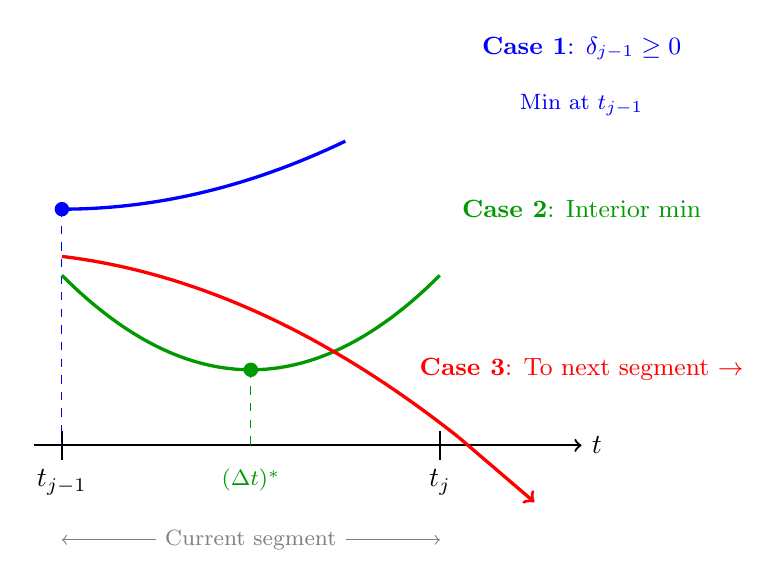
\begin{tikzpicture}[scale=1.2]
    \draw[->, thick] (-0.3, 0) -- (5.5, 0) node[right] {$t$};
    
    % Tick marks for t_{j-1} and t_j
    \draw[thick] (0, 0.15) -- (0, -0.15) node[below] {$t_{j-1}$};
    \draw[thick] (4, 0.15) -- (4, -0.15) node[below] {$t_j$};
    
    % Segment bracket (lowered)
    \draw[<->, gray] (0, -1.0) -- (4, -1.0) node[midway, fill=white, font=\footnotesize] {Current segment};
    
    % === CASE 1: Increasing from start (blue) ===
    \draw[blue, very thick, domain=0:3, smooth, samples=50] plot (\x, {0.08*\x*\x + 2.5});
    \filldraw[blue] (0, 2.5) circle (2pt);
    \draw[blue, dashed] (0, 2.5) -- (0, 0);
    \node[blue, font=\small] at (5.5, 4.2) {\textbf{Case 1}: $\delta_{j-1} \ge 0$};
    \node[blue, font=\footnotesize] at (5.5, 3.6) {Min at $t_{j-1}$};
    
    % === CASE 2: Minimum inside (green) ===
    \draw[green!60!black, very thick, domain=0:4, smooth] plot (\x, {0.25*(\x-2)*(\x-2) + 0.8});
    \filldraw[green!60!black] (2, 0.8) circle (2pt);
    \draw[green!60!black, dashed] (2, 0.8) -- (2, 0);
    \node[below, green!60!black, font=\footnotesize] at (2, -0.15) {$(\Delta t)^*$};
    \node[green!60!black, font=\small] at (5.5, 2.5) {\textbf{Case 2}: Interior min};
    
    % === CASE 3: Decreasing throughout (red) ===
    \draw[red, very thick, domain=0:4.2, smooth, samples=50] plot (\x, {2.0 - 0.08*\x*\x - 0.12*\x});
    \draw[->, red, very thick] (4.2, {2.0 - 0.08*4.2*4.2 - 0.12*4.2}) -- (5.0, {2.0 - 0.08*5.0*5.0 - 0.12*5.0});
    \node[red, font=\small] at (5.5, 0.8) {\textbf{Case 3}: To next segment $\to$};
    
\end{tikzpicture}
\caption{Search for the Cauchy Point: the three possible cases during the minimization of $q(x(t))$ over a segment $[t_{j-1}, t_j]$.}
\label{fig:cauchy-search-cases}
\end{figure}

\begin{figureexplanation}
On each linear segment of the projected trajectory, the objective function $q(x(t))$ is a parabola (quadratic function of $t$).
\begin{itemize}
    \item \textbf{Case 1 (Blue)}: The slope is upward from the start. The minimum on the segment is the starting point $t_{j-1}$. This is the Cauchy Point.
    \item \textbf{Case 2 (Green)}: The parabola reaches its minimum inside the segment (the derivative vanishes at $(\Delta t)^* < t_j - t_{j-1}$). This is the Cauchy Point.
    \item \textbf{Case 3 (Red)}: The function decreases throughout the segment. The minimum is not reached here, we must continue the search on the next segment (beyond $t_j$).
\end{itemize}
\end{figureexplanation}

\begin{center}
\begin{tikzpicture}[scale=1.4]
    % 3D Box (parallélépipède) - perspective isométrique
    % On utilise d comme unité de base pour les arêtes
    \def\d{2.5}  % taille d'une arête
    
    % Coordonnées des 8 sommets du cube
    % Face avant : coins (0,0), (d,0), (d,d), (0,d)
    % Face arrière : décalage de (0.6d, 0.4d) en perspective
    \def\px{0.6}  % facteur de perspective x
    \def\py{0.4}  % facteur de perspective y
    
    % Face avant (rouge)
    \draw[red, thick] (0,0) -- (\d,0) -- (\d,\d) -- (0,\d) -- cycle;
    
    % Face droite (rouge)
    \draw[red, thick] (\d,0) -- (\d+\d*\px, \d*\py) -- (\d+\d*\px, \d+\d*\py) -- (\d,\d) -- cycle;
    
    % Face supérieure (rouge)
    \draw[red, thick] (0,\d) -- (\d,\d) -- (\d+\d*\px, \d+\d*\py) -- (\d*\px, \d+\d*\py) -- cycle;
    
    % Arêtes arrière (pointillés rouges)
    \draw[red, thick, dashed] (0,0) -- (\d*\px, \d*\py);
    \draw[red, thick, dashed] (\d*\px, \d*\py) -- (\d*\px, \d+\d*\py);
    \draw[red, thick, dashed] (\d*\px, \d*\py) -- (\d+\d*\px, \d*\py);
    
    % Centre du cube (point x)
    \coordinate (center) at (\d/2 + \d*\px/2, \d/2 + \d*\py/2);
    \fill[blue] (center) circle (2.5pt);
    \node[blue, below] at (center) {$t_x$};
    
    % X' = milieu de l'arête supérieure GAUCHE (arête entre (0,d) et (d*px, d+d*py))
    \coordinate (Xprime) at (\d*\px/2, \d + \d*\py/2);
    
    % X'' = au-dessus de l'arête du fond (arête arrière supérieure)
    % L'arête arrière va de (d*px, d+d*py) à (d+d*px, d+d*py)
    % On place X'' au-dessus du milieu de cette arête
    \coordinate (Xpp) at (\d*\px + \d*0.8, \d + \d*\py + \d*0.5);
    
    % X = intersection de la droite (center -> X'') avec la face supérieure
    % On calcule où la ligne center-X'' coupe le plan z=d (face sup)
    % La face sup a y entre d et d+d*py selon la perspective
    % Approximation: X est sur le segment center-X'' quand on atteint la hauteur de la face sup
    \coordinate (X) at ($(center)!0.40!(Xpp)$);  % X plus haut sur la trajectoire
    \fill[black] (X) circle (2pt);
    
    % Trajectoire x - tg : du centre (center) vers X'' - en teal
    \draw[very thick, teal] (center) -- (X);
    \draw[->, very thick, teal] (X) -- (Xpp);
    \node[teal, left] at (Xpp) {$x-tg$};
    
    % L'arête supérieure arrière va de (d*px, d+d*py) à (d+d*px, d+d*py)
    % L'arête de droite de la face supérieure va de (d,d) à (d+d*px, d+d*py) avec direction (d*px, d*py)
    % Pour que la ligne X→MidBack soit parallèle à cette arête, on suit la direction (px, py)
    % MidBack doit être sur l'arête arrière, donc à y = d+d*py
    % Le facteur dépend de la distance entre X et l'arête arrière
    \coordinate (MidBack) at ($(X) + (0.55*\d*\px, 0.55*\d*\py)$);
    
    % Ligne de X vers le point sur l'arête arrière (parallèle à l'arête de droite)
    \draw[black, very thick] (X) -- (MidBack);
    
    % Coin supérieur arrière droit
    \coordinate (EdgePoint) at (\d+\d*\px, \d+\d*\py);
    
    % Ligne le long de l'arête supérieure arrière vers le coin (confondue avec l'arête)
    \draw[black, very thick] (MidBack) -- (EdgePoint);
    
\end{tikzpicture}
\captionof{figure}{Trajectory projected onto the feasible box (3D). The trajectory $x-tg$ crosses the cube and exits through the top face at $X$, then follows the edges (projection).}
\end{center}

\begin{figureexplanation}
\textbf{The Cauchy Path:}
This 3D figure illustrates the path $x(t) = P(x - tg)$.
\begin{itemize}
    \item Initially (center), we follow the steepest descent direction $-g$ (straight line).
    \item As soon as we hit a face of the box (here the top face), we can no longer "go up". Projection forces us to stay on the face.
    \item Then we continue to slide on the face, or along an edge, until we find a local minimum along this broken path. This minimum is the \textbf{Cauchy Point} $x^c$.
\end{itemize}
\end{figureexplanation}

\subsubsection{Step 2: Minimization in the Subspace}

Once $x^c$ is computed, we work on the active set:
\begin{equation}
    \mathcal{A}(x^c) = \{ i \mid x_i^c = l_i \text{ or } x_i^c = u_i \}
\end{equation}

We approximately solve the QP problem by \textbf{fixing} $x_i$ to $x_i^c$ for $i \in \mathcal{A}(x^c)$.
The other components are determined by:
\begin{equation}
    \min_{x \in \mathbb{R}^n} q(x) = \frac{1}{2} x^\top G x + c^\top x
\end{equation}
subject to:
\begin{equation}
    \begin{cases}
        x_i = x_i^c & \text{if } i \in \mathcal{A}(x^c) \\
        l_i \le x_i \le u_i & \text{if } i \notin \mathcal{A}(x^c)
    \end{cases}
\end{equation}

\begin{remarque}
    It is not necessary (nor desirable) to solve this subproblem exactly. We only need to find a point that is better than $x^c$.
    For example, we can use a Conjugate Gradient algorithm (as in Section~\ref{chap:unconstrained}) and stop as soon as the constraints $l_i \le x_i \le u_i$ for $i \notin \mathcal{A}(x^c)$ are satisfied.
\end{remarque}

\begin{remarque}
    In principle, the algorithm can be used for general inequality constraints $a_i^\top x \ge b_i$, but significantly more complex calculations are needed.
    For instance, to find the projection of a point $x$ onto the feasible set, one must solve:
    \begin{equation}
        \min_{\bar{x} \in \mathbb{R}^n} \|x - \bar{x}\|^2, \quad \text{subject to } a_i^\top \bar{x} \ge b_i, \; \forall i \in \mathcal{I}
    \end{equation}
    which can be as difficult as the original problem.
    
    \textbf{Solutions:} resort to active-set methods or interior-point methods.
\end{remarque}

\subsubsection{Summary}

\begin{algorithm}[H]
    \caption{Projected gradient method for Quadratic Programming}
    \SetAlgoLined
    Compute a feasible starting point $x_0$\;
    \For{$k=0, 1, \ldots$}{
        \If{$x_k$ satisfies the KKT conditions for the bound-constrained problem}{
            \Stop with solution $x^*=x_k$\;
        }
        Set $x=x_k$ and find the Cauchy point $x^c$\;
        Find an approximate solution $x^+$ to
        \begin{align*}
            \min_{x} q(x)=\frac{1}{2}x^\top Gx &+ x^\top c\\
            \text{subject to } x_i&=x_i^c, \quad i\in\mathcal{A}(x^c)\\
            l_i \leq x_i & \leq u_i, \quad i\notin\mathcal{A}(x^c)
        \end{align*}
        such that $q(x^+)\leq q(x^c)$ and $x^+$ is feasible\;
        $x_{k+1}\leftarrow x^+$\;
    }
\end{algorithm}

%%%%%%%%%%%%%%%%%%%%%%%%%%%%%%%%%%%%%%%%%%%%%%%%%%%%%%%%%%%%
\section{Practice Exercises (Nocedal \& Wright)}
\label{sec:11.exercises}

These exercises correspond to chapter 16 (Quadratic Programming) of the reference book.

\bigskip
\begin{exercice}[KKT Conditions for QP]
Write the KKT conditions for the convex quadratic program with mixed constraints:
\begin{align*}
    \min_x \quad & \frac{1}{2} x^\top G x + x^\top c \\
    \text{s.t. } \quad & Ax \ge b \\
               & \bar{A}x = \bar{b}
\end{align*}
Use these conditions to derive an analogue of the generic primal-dual system.
\end{exercice}

\begin{correction}
Lagrangian:
$$ L(x, \lambda, \mu) = \frac{1}{2}x^\top G x + c^\top x - \lambda^\top (Ax - b) - \nu^\top (\bar{A}x - \bar{b}). $$
KKT Conditions:
1. Stationarity: $Gx + c - A^\top \lambda - \bar{A}^\top \nu = 0$.
2. Primal Feasibility: $Ax \ge b$, $\bar{A}x = \bar{b}$.
3. Dual Feasibility: $\lambda \ge 0$.
4. Complementarity: $\lambda_i (A_i x - b_i) = 0, \forall i$.
\end{correction}
\bigskip

\bigskip
\begin{exercice}[Resolution by Active-Set]
Program (or manually unroll) the Active-Set algorithm to solve:
\begin{align*}
    \min_{x_1, x_2} \quad & x_1^2 + 2x_2^2 - 2x_1 - 6x_2 - 2x_1 x_2 \\
    \text{s.t. } \quad & \frac{1}{2}x_1 + \frac{1}{2}x_2 \le 1 \\
               & -x_1 + 2x_2 \le 2 \\
               & x_1 \ge 0, x_2 \ge 0
\end{align*}
Test with several starting points (interior, vertex, non-vertex boundary).
\end{exercice}

\begin{correction}
This is an implementation exercise for Algorithm 16.3.
You have to start from a feasible point $x_0$, identify the active set $\mathcal{W}_0$.
Solve the equality subproblem. Compute multipliers. If $\lambda_i < 0$ for an active constraint, relax it.
(Specific solution depends on the chosen starting point).
\end{correction}
\bigskip

\bigskip
\begin{exercice}[Graphical Example and Resolution]
Consider the QP problem:
\begin{align*}
    \max \quad & 6x_1 + 4x_2 - 13 - x_1^2 - x_2^2 \\
    \text{s.t. } \quad & x_1 + x_2 \le 3 \\
               & x_1 \ge 0, x_2 \ge 0
\end{align*}
\begin{enumerate}
    \item Solve this problem graphically.
    \item Apply the Active-Set method to find the solution.
\end{enumerate}
\end{exercice}

\begin{correction}
Minimize $f(x) = (x_1 - 3)^2 + (x_2 - 2)^2$ (by completing the squares and changing the sign of max).
The unconstrained minimum is $(3, 2)$.
Constraint $x_1 + x_2 \le 3$. The point $(3,2)$ has $3+2=5 > 3$, so it is not feasible.
The point closest to $(3,2)$ on the line $x_1+x_2=3$ (in the positive quadrant) is the solution.
Projection of $(3,2)$ onto $x_1+x_2-3=0$:
Normal vector $(1,1)$. Line passing through $(3,2)$: $(3+t, 2+t)$.
Intersection: $(3+t) + (2+t) = 3 \implies 2t + 5 = 3 \implies 2t = -2 \implies t=-1$.
Projected point: $(2, 1)$.
This point satisfies $x \ge 0$. So $x^*=(2,1)$.
\end{correction}
\bigskip

\bigskip
\begin{exercice}[Null-Space Method ($p_Y, p_Z$) - Exam Type]
Consider the following equality QP problem (analogous to one iteration of an EQP):
\begin{align*}
    \min_{p} \quad & \frac{1}{2} p^\top G p + g^\top p \\
    \text{s.t. } \quad & A p = -h
\end{align*}
with $G = \begin{pmatrix} 4 & 0 \\ 0 & 2 \end{pmatrix}$, $A = \begin{pmatrix} 1 & 1 \end{pmatrix}$, $h = -2$, $g = \begin{pmatrix} -1 \\ -1 \end{pmatrix}$.
\begin{enumerate}
    \item Construct a matrix $Z$ (basis of the null space of $A$) and a matrix $Y$ (such that $AY$ is invertible, or pseudo-inverse).
    \item Write the decomposition $p = Y p_Y + Z p_Z$.
    \item Calculate $p_Y$ by solving $AY p_Y = -h$.
    \item Write the reduced system for $p_Z$: $(Z^\top G Z) p_Z = -(Z^\top g + Z^\top G Y p_Y)$ and solve it.
    \item Deduce the optimal step $p$.
\end{enumerate}
\end{exercice}

\begin{correction}
\textbf{1. Construction of Y and Z:}
Linear constraint $p_1 + p_2 = 2$ (since $Ap = -(-2) = 2$).
$A = \begin{pmatrix} 1 & 1 \end{pmatrix}$. Basis of the null space ($\ker A$): we look for $z$ such that $z_1 + z_2 = 0$.
Let's set $Z = \begin{pmatrix} 1 \\ -1 \end{pmatrix}$.
For $Y$, we look for $y$ such that $Ay = I$ (here $1$). Let's choose $Y = \begin{pmatrix} 1/2 \\ 1/2 \end{pmatrix}$ (Pseudo-inverse) or $Y = \begin{pmatrix} 1 \\ 0 \end{pmatrix}$.
Let's take the simple choice from the course (often $Y = A^\top (AA^\top)^{-1}$). $AA^\top = 2$, so $Y = \begin{pmatrix} 1/2 \\ 1/2 \end{pmatrix}$.
Check: $A Z = 1(1) + 1(-1) = 0$. $A Y = 1(1/2) + 1(1/2) = 1$. OK.

\textbf{2. Decomposition:} $p = Y p_Y + Z p_Z$.

\textbf{3. Calculation of $p_Y$:}
$AY p_Y = -h \implies 1 \cdot p_Y = 2 \implies p_Y = 2$.
So the range space component contributes $Y p_Y = \begin{pmatrix} 1 \\ 1 \end{pmatrix}$.
The point $\begin{pmatrix} 1 \\ 1 \end{pmatrix}$ indeed satisfies the constraint $1+1=2$.

\textbf{4. Calculation of $p_Z$:}
Reduced matrix $Z^\top G Z = \begin{pmatrix} 1 & -1 \end{pmatrix} \begin{pmatrix} 4 & 0 \\ 0 & 2 \end{pmatrix} \begin{pmatrix} 1 \\ -1 \end{pmatrix} = \begin{pmatrix} 1 & -1 \end{pmatrix} \begin{pmatrix} 4 \\ -2 \end{pmatrix} = 4 + 2 = 6$.
Reduced vector $Z^\top g = \begin{pmatrix} 1 & -1 \end{pmatrix} \begin{pmatrix} -1 \\ -1 \end{pmatrix} = -1 + 1 = 0$.
Cross term $Z^\top G Y p_Y = \begin{pmatrix} 1 & -1 \end{pmatrix} \begin{pmatrix} 4 & 0 \\ 0 & 2 \end{pmatrix} \begin{pmatrix} 1 \\ 1 \end{pmatrix} = \begin{pmatrix} 1 & -1 \end{pmatrix} \begin{pmatrix} 4 \\ 2 \end{pmatrix} = 4 - 2 = 2$.
Reduced equation: $6 p_Z = -(0 + 2) \implies p_Z = -2/6 = -1/3$.

\textbf{5. Solution $p$:}
$p = \begin{pmatrix} 1 \\ 1 \end{pmatrix} + \begin{pmatrix} 1 \\ -1 \end{pmatrix} (-1/3) = \begin{pmatrix} 1 - 1/3 \\ 1 + 1/3 \end{pmatrix} = \begin{pmatrix} 2/3 \\ 4/3 \end{pmatrix}$.
Check: $p_1 + p_2 = 6/3 = 2$. OK.
\end{correction}
\bigskip

\bigskip
\begin{checkpoint}
\begin{itemize}
    \item \textbf{QP KKT:} Write the KKT system for an equality-constrained QP problem.
    \item \textbf{Null Space:} How to decompose the step $p$ into $p_Y$ and $p_Z$? Which one minimizes the reduced quadratic?
    \item \textbf{Active Set:} How does this method handle inequalities? (By adding/removing constraints from the working set).
\end{itemize}
\end{checkpoint}
